\documentclass{beamer}

\usepackage[frenchb]{babel}
\usepackage[T1]{fontenc}
\usepackage[utf8]{inputenc}
\usepackage{graphicx} %pour l'intégration d'images
%\usepackage{tikz} %pour la création de figures
%\usepackage{indentfirst} %pour indenter du texte
%\usepackage{fancyhdr} %pour les headers et footers
%\usepackage{array} %pour les tableaux
%\usepackage{amssymb} %pour les "checkmarks"

%\usepackage{fullpage}
%\usepackage{microtype}
%\usepackage{wrapfig}

%\hypersetup{pdfpagemode=FullScreen} %ligne à décommenter pour le PDF final

\newcommand{\HRule}{\rule{\linewidth}{0.1mm}}

\frenchbsetup{StandardLists=true} %permet d'utiliser des ronds comme puces principales dans les listes

\usetheme{Warsaw}

\title{CPU}
\author{Alexandre Faucher, Gada Rezgui}

\begin{document}

%%%%%%%%%% Page de garde %%%%%%%%%%

\begin{frame}
	\begin{center}

	{\Huge \textbf{Soutenance de projet}}

	\vspace*{0.3cm}

	{\large \textbf{Architecture des Ordinateurs}}

	\vspace*{0.5cm}

	\textit{Réalisé par :}

	{\large \textbf{Alexandre FAUCHER\\ Gada REZGUI}}

	\vspace*{0.5cm}

	\textit{Jury :}

	{\large \textbf{Benoît MIRAMOND}}

	\vspace*{0.5cm}

	{\large 8 avril 2015}

	\end{center}
\end{frame}

%%%%%%%%%% Table des matières %%%%%%%%%%

%\tableofcontents

\begin{frame}
\frametitle{Table des matières}
\begin{enumerate}
	\item Introduction
	\item Ressources

	\item Unité de contrôle
	\item Problèmes rencontrés


\end{enumerate}
\end{frame}

%%%%%%%%%% Contenu %%%%%%%%%%

%\section{Introduction}
\begin{frame}
\frametitle{Introduction}
\begin{block}{Contexte}

		 Prolongation du projet fait en L2

\end{block}
\begin{block}{Spécification}
	\begin{itemize}
		\item Processeur 16 bits
		\item 5 opérations
		\item Encodage des données en complément à deux
		\item Entièrement générique : processeur n bits possible
	\end{itemize}
\end{block}
\end{frame}

%\section{Ressources}
\begin{frame}
\frametitle{Ressources} %logisim, GHDL, EDA Playground
						%+fac = Quartus Altera, cartes FPGA
\begin{block}{Programmation}
	\begin{itemize}
		\item EDA Playground
		\item GHDL
	\end{itemize}
\end{block}
\begin{block}{Simulation}
	\begin{itemize}
		\item GTKWave
	\end{itemize}
\end{block}
\end{frame}



%\section{Unité de contrôle}
\begin{frame}
\frametitle{Unité de contrôle}
Machine de Moore
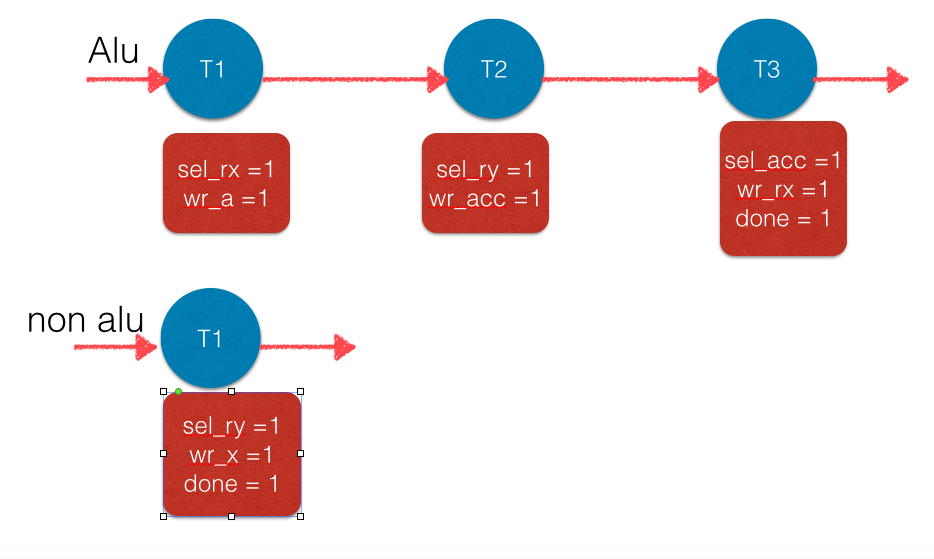
\includegraphics[scale=0.35]{fsm}
\end{frame}

%\section{Problèmes rencontrés}
\begin{frame}
\frametitle{Problèmes rencontrés}
\begin{block}{Ressources}
	\begin{itemize}
		\item Quartus II \& Modelsim laborieux à installer
		\item Indisponible sur MacOS
		\item GHDL \& GTKWave : nécessite du temps pour apprendre
		\item Perte d'une partie du projet effectuée en TD
	\end{itemize}
\end{block}
\begin{block}{Méthode}
	\begin{itemize}
		\item Concentration sur la compilation
		\item Peu de tests unitaires : effet tunnel
	\end{itemize}
\end{block}
\end{frame}


\begin{frame}
\begin{center}
	{\Large \textbf{Avez-vous des questions?}}
\end{center}
\end{frame}



%%%%%%%%%% Slides surprise %%%%%%%%%%

\end{document}
